\documentclass[11pt]{article}
\usepackage[nottoc, numbib]{tocbibind}
\usepackage[fleqn]{amsmath}
\usepackage{epigraph}
\usepackage{amssymb}
\usepackage{amsmath}
\usepackage{bm}
\usepackage{mathrsfs}
\usepackage{graphicx}
\usepackage{float}
\usepackage{subcaption}
\usepackage{relsize}
\usepackage{listings}
\usepackage{tikz}
\usepackage{natbib}
%\usepackage{breqn}
\lstset{language=Python,
    frame=single,
    breaklines=true,
    postbreak=\raisebox{0ex}[0ex][0ex]{\ensuremath{\color{red}\hookrightarrow\space}}
}
%%\usepackage[margin=2cm]{geometry}
%%\floatstyle{boxed}
\restylefloat{figure}
\newcommand{\Prop}{\textbf{Proposition: }}
\newcommand{\Prob}{\textbf{Problem: }}
\newcommand{\Prf}{\textbf{Proof: }}
\newcommand{\Sol}{\textbf{Solution: }}
\newcommand{\grad}{\nabla}
\newcommand{\Nats}{\mathbb{N}}
\newcommand{\Ints}{\mathbb{Z}}
\newcommand{\Rats}{\mathbb{Q}}
\newcommand{\Reals}{\mathbb{R}}
\newcommand{\Comps}{\mathbb{C}}
\newcommand{\Prb}[1]{P\left( #1 \right)}
\newcommand{\PT}[1]{P\left( \text{#1} \right)}
\newcommand{\PCon}[2]{P\left( #1 \mid #2 \right)}
\newcommand{\PConT}[2]{P\left( \text{#1} \mid \text{#2} \right)}
\DeclareMathOperator{\E}{\mathbb{E}}
\DeclareMathOperator{\tr}{\textbf{tr}}
\DeclareMathOperator*{\argmin}{argmin}
\DeclareMathOperator*{\argmax}{argmax}
\newcommand{\thus}{\quad\mathlarger{\mathlarger{\mathlarger{\Rightarrow}}}\quad} 
\newcommand{\wght}{\mathbf{w}}
\newcommand{\im}{\text{im }}
\usepackage[left=2cm,right=2cm,top=2cm,bottom=2cm,nohead]{geometry}
%%\newcommand\scalemath[2]{\scalebox{#1}{\mbox{\ensuremath{\displaystyle #2}}}}
\setlength\parindent{0pt}
\parskip = \baselineskip

\usetikzlibrary{shapes,arrows}

\tikzstyle{block} = [rectangle, draw, thick, align=center, rounded corners]
\tikzstyle{boundingbox} = [very thick, dotted, gray]
\tikzstyle{dashblock} = [rectangle, draw, thick, align=center, dashed]
\tikzstyle{conc} = [ellipse, draw, thick, dashed, align=center]
\tikzstyle{netnode} = [circle, draw, very thick, inner sep=0pt, minimum size=0.5cm]
\tikzstyle{relunode} = [rectangle, draw, very thick, inner sep=0pt, minimum size=0.5cm]
\tikzstyle{line} = [draw, very thick, -latex']

\begin{document} 
\title{ARRR: Transfer and flexibility}
\author{Andrew Lampinen}
\date{3/13/2019}
\maketitle

\newpage
\tableofcontents

\newpage
\section{Introduction}
\epigraph{``The most elementary single difference between the human mind and that of brutes lies in this deficiency on the brute's part to associate ideas by similarity.''}{William James, \textit{Principles of Psychology}}
Deep learning methods have achieved incredible success recently, achieving human level performance in domains ranging from vision \citep[e.g.]{Szegedy2015} to playing games \citep[e.g.]{Silver2016}. Yet these systems lack some important human abilities \citep[e.g.]{Lake2016}. Deep learning models are data-hungry, while humans can frequently learn from relatively few examples. Furthermore, even if they are given a large amount of data, deep learning systems may not be able to generalize well outside the data distribution they trained on. Finally, once knowledge is learned in the weights of a deep learning model, it is difficult to flexibly reuse that knowledge. From the perspective of William James (quoted above), most neural networks are brutes, which don't understand the similarity of new situations to their prior experiences, and so do not know how to flexibly respond to changes in their environment or goals. \par
By contrast, humans can use our knowledge flexibly. We can learn from few examples. We can introspect about our learned behavior to explain or change it. We can even remap our behavior in a way completely inconsistent with our prior behavior, such as trying to lose a game we have previously been trying to win \citep{Lake2016}. More generally, we are often able to accurately behave according to linguistic instructions without seeing examples of such behavior. All of these types of flexibility can be quite difficult for deep learning systems. \par 
This apparent contrast between humans and neural networks has raised questions about the validity of neural networks as a cognitive model for many years \citep[e.g.]{Fodor1988}, and the recent successes of deep learning have only increased the frequency of these critiques \citep[e.g.]{Lake2015, Lake2016, Lake2017, Marcus2018}. It is important to address these perspectives, and to understand how deep learning systems can be improved to serve as better models of human flexibility. There have been a number of attempts to address or integrate these critiques from a variety of perspectives \citep[e.g.]{McClelland1999, McClelland2010}. In this paper, I will particularly focus on how these critiques overlook the benefits of transfer \citep{Lampinen2017a} and recent progress in deep learning \citep{Hansen2017}. In particular, deep learning research has made important progress on improving learning speed, generalization, and flexibility. However, even with contemporary methods there are many human-like abilities that remain frustratingly out of reach. \par
In the remainder of this paper, I will first review some of the cognitive issues and the progress to date and try to provide a unifying perspective on how various types of transfer contribute to human learning and flexibility. I will then show some of my prior research and present directions on this topic, including analyses of the effects of transfer in neural networks, explorations of flexibility and transfer in humans, and a new type of deep learning architecture that yields much greater flexibility. \par

\section{Area review: Cognitive flexibility}

What kind of flexibility do humans have? We are often able to learn rapidly. For example, we can achieve some competence in a novel video game within a few minutes \citep{Lake2016}. We can learn new concepts from seeing only a relatively small number of examples \citep[e.g.]{Bourne1970}. We can often learn even faster if we can actively participate in the learning process by selecting examples rather than passively receiving them, especially if the concepts are simple enough that we can generate a good hypothesis space \citep{Markant2014a}. \par
We can then apply what we have learned to new situations. The studies of \citet{Bourne1970} that I referenced above show that once people have learned a new concept from examples, they can generalize that knowedge to learn structurally-similar new concepts more rapidly. Indeed, even without explicit awareness of the relationship between two tasks, humans can sometimes benefit from transfer effects \citep[e.g.]{Day2011}. In general, human analogical transfer abilities have been suggested to be a critical component of `` what makes us smart'' \citep{Gentner2003}. \par
Yet human flexibility is apparent beyond transfer between isomorphic tasks. We can often competently change our learned behavior in response to instruction or other goals, such as trying to lose a game we were previously trying to win, or trying to achieve some orthogonal task \citep{Lake2016}. Indeed, it has been known for almost a century that even other animals exhibit this sort of flexible knowledge use -- they engage in ``latent learning'' of environmental features that may be useful when solving future tasks \citep{Blodgett1929}. Humans are capable of flexibly applying our knowledge in many situations. \par
However, human flexibilty is not universal. Sometimes it is quite difficult for us to integrate new knowledge. For example, even undergraduate students with substantial mathematical background often struggle with understanding new mathematical concepts. They may mistakenly assume the converse of a theorem, or get caught up in concrete ways of thinking about abstract concepts \citep{Hazzan1999}. Socrates' dialog about doubling the area of a square captures the misunderstandings that even modern subjects make, yet it does not help them to deeply understand the principle \citep{Goldin2011}. Even after engaging with the dialog, nearly 50\% of modern subjects failed at the simplest generalization of the principle: to a square of different size. Similarly, even students who complete a course in geometry in high school may not achieve formal deductive understanding of the concepts taught unless (or until) they become undergraduate mathematics majors \citep{Burger1986}. Furthermore, superficial details of how a concept is presented can have profound impacts on how easy it is to reason about, even if the underlying concept is exactly the same \citep[e.g.]{Kotovsky1985, Kaminski2008, Lampinen2017b}. There is a wealth of research showing that our learning is far from universally flexible. \par 
We also often fail to flexibly use the knowledge we have. For example, even mathematics students who can correctly state a rule or theorem are not necessarily able to apply it to create a proof \citep{Weber2001}. Similarly, even if experimental subjects can learn a basic concept rapidly, it may be difficult for them to apply it in more abstract situations or to extract more formal understanding from it \citep[e.g.]{Lampinen2017b}. Likewise, rapid analogical transfer is often only possible when superficial details match closely, or when subjects are explicitly told to transfer \citep[e.g.]{Gick1980}. Because of findings like these, \citet{Detterman1993} has argued that inducing transfer requires manipulations ``with the subtlety of a baseball bat,'' and so we should conclude that ``significant transfer is probably rare and accounts for very little human behavior.'' This is a particularly tendentious presentation of the issues, but it captures the important broader insight that humans are not always rapid learners or flexible reasoners. \par 
How can we reconcile the demonstrations of rapid learning and flexibility with the evidence that some concepts are learned slowly and some knowledge is inflexible? How can we reconcile arguments that transfer is key to ``what makes us smart'' \citep{Gentner2003}, with arguments that ``significant transfer is probably rare and accounts for very little human behavior'' \citep{Detterman1993}? There are a variety of factors that contribute to transfer. We need high-quality representations of the concepts we are learning in order to reason flexibly with them. These generalizable representations are generally created through making connections between different pieces of our knowledge \citep{Wilensky1991, Schwartz2015}. Relatedly, we often need strategic meta-knowledge about where and how to apply our knowledge in new situations, which also must be learned \citep{Weber2001}. Both these factors mean that transfer may happen more easily over longer periods of time, as I have argued in my prior work \citep{Lampinen2017a}. The quality of the representations we have, and the way those representations relate to the new tasks we are presented with, both affect our ability to learn rapidly and reason flexibly. \par 

\subsection{Flexibility as transfer}
I argue that all these types of flexibility (and inflexibility) can be seen as transfer, defined broadly as the way that ``knowledge acquired in one situation applies (or fails to apply) in other situations.'' \citep{Singley1989}. From this definition it is clear that applying learned features and structures to learn faster in a new situation, as in \citet{Bourne1970} is a type of transfer. However, I argue that all rapid learning must rely on transfer of prior knowledge in order to constrain the hypothesis space under consideration. Even other types of flexibility, such as adapting to instructions, can be seen as transferring several different types of knowledge (prior knowledge about a task, other related taks, and language) to a new situation. For example, if we are asked to try to lose at chess, we are essentially presented a new task to which we need to transfer both our prior knowledge of chess and our prior knowledge of ``trying to lose'' means. Thus flexibility and transfer are essentially two perspectives on the same broad phenomena. I will therefore use ``flexibility'' generally to refer to the behavioral phenomena, and ``transfer'' to refer to the computational principles underlying these phenomena. \par  
Why do we sometimes fail to be flexible? I think there are several reasons this can occur. First, we may not have the prior knowledge necessary to be flexible. We can't transfer what we don't know. Second, our representations may lack the quality necessary to transfer them. We often can't transfer what we don't know well \citep[c.f.]{Hazzan1999, Weber2001}. Third, we may not recognize that we have applicable prior knowledge to transfer \citep{Detterman1993}. Finally, we may actually have prior beliefs that do not apply to the present situation, and so transferring them will actually interfere with our ability to learn. This is generally called ``negative transfer'' \citep{Singley1989}. \par
For transfer to be beneficial overall, we must generally encounter settings where our prior knowledge is applicable, and furthermore we must have good ways of integrating that prior knowledge with new experiences. In the next section I will discuss some of the features that allow us to do so. \par

\subsection{What factors contribute to our flexibility?}
We need to address the computational question of how and when we can transfer our knowledge to behave flexibly. In this section I will give a brief overview of the contributing factors. \par 

\textbf{Complementary learning systems:} First, it has been proposed that we have complementary learning systems \citep{McClelland1995, Kumaran2016}. These complementary systems allow us to learn rapidly from new knowledge while avoiding catastrophic interference \citep{McCloskey1989} with the statistical knowledge we have accumulated over longer timescales. The key idea is that we have a slow (parametric) learning system which sets up good representations, while a fast (nonparamteric) learning system stores new knowledge by using these representations. Throughout this paper, we will return to this theme of fast and slow learning which support each other. I will therefore divide the rest of this section into the ``slow'' and ``fast'' systems that contribute to transfer. \par
\subsubsection{Slow}
\textbf{Culture \& education:} One critical contributor to transfer is culture. Our cultures have accumulated knowledge over extremely long time scales that allows us to advance much more rapidly now \citep{Bengio2012}. Before they graduate high school, many children in the US gain fluency in concepts like calculus that took millenia to discover. Because culture has set up useful representations for these concepts, we are able to acquire them much more rapidly \citep[e.g.]{McClelland2016}. Furthermore, the systems of education that culture has set up are structured in an attempt to help us learn and generalize most effectively. \par 
\textbf{Transfer between tasks:} Even if culture has not explicitly highlighted (or engineered) structural relationships between tasks, we can benefit from structural similarity. For example, after learning an artificial grammar, subjects can generalize their knowledge to novel sequences from the same grammar applied to novel symbols \citep[e.g.]{Tunney2001}. From learning about simple harmonic oscillators in the context of springs, participants can transfer to a superficially unrelated problem about controlling the population of a city \citep[e.g.]{Day2011}. Because many tasks we perform share deep underlying structures, we can take advantage of transfer to learn faster on new tasks. \par 
\textbf{Grounding and representation quality:} One particular type of transfer that seems to be especially useful is grounding \citep{Barsalou2007}. In particular, conceptual representations often tend to be tied into more basic perceptual-motor systems, e.g. arithmetic in the Approximate Number System \citep{Park2013}, or mathematical (and other) reasoning in gestures \citep{Goldin-Meadow1993, Goldin-Meadow1999}. This sort of grounding can be very beneficial to understanding \citep{Nathan2008, Wakefield2018}. Because our perceptual-motor system have exceptionally good representations that are trained over long developmental time-scales, we may benefit from leveraging these representations to transfer our understanding to analogous conceptual domains. \par 
At the same time, grounding can hold us back. Even our understanding of symbolic expressions seems to be influenced by ``meaningless'' perceptual details like their spacing \citep{Landy2007}. It has also been argued that too concrete of examples can limit generalization \citep{Kaminski2008}, although the details of that particular demonstration have been debated \citep{DeBock2011, Lampinen2017b}. There is probably some negative transfer from grounding in some cases, but overall it is probably outweighed by the positive. \par
\textbf{Rerepresentation:} The work of Annette Karmiloff-Smith \citep[e.g.]{Karmiloff-Smith1986, Karmiloff-Smith1992, Clark1993} focused on the idea that we repeatedly redescribe our internal knowledge, reorganizing it in order to better understand the world. To support this theory, she examined evidence of U-shaped developmental curves, where children would actually get worse at a task before they reached ceiling, often because they at first over-generalized a rule. She argues that this shows a pattern of systematic progression of knowledge from implicit representations to various stages of explicit ones which allow progressively more flexibility. In \citet{Karmiloff-Smith1986} she describes some particularly interesting evidence: children fail to balance an oddly shaped block when asked to do so, but successfully balance it when asked to build a house, because their procedural knowledge is more sophisticated than their explicit knowledge. \par 
This pattern of procedural knowledge proceeding more explicit or object-like knowledge is supported by a much broader literature, from the gesture results of \citet{Goldin-Meadow1993} referenced above to work suggesting that we progress from understanding mathematical concepts as processses to understanding them as objects \citep{Dubinsky1991, Hazzan1999}. If we do not already have good representations for a concept, we must create them by slow, procedural learning and reorganization, before we can begin to reason flexibly with the concept. \par 
\textbf{Summary:} We accumulate knowledge throughout the course of our lives. Some of this knowledge is implicit in the statistics of the world around us, while some is culturally constructed and transmitted. The quality of our representations of this knowledge can be improved by connecting it to other knowledge, or by grounding it in perceptual-motor understanding. Once we have acquired sufficiently high-quality representations of this knowledge, we are often able to transfer it when we encounter a new task, and thereby learn more effectively than we could from \textit{tabula rasa}. This improvement in learning manifests as both more efficient learning and better generalization. \par

\subsubsection{Fast}
In this section I will discuss the systems that contribute to fast learning and transfer. It's important to note that these are systems that can be applied rapidly, but not necessarily learned rapidly. Indeed, many of these reasoning systems must themselves be learned over development. \par
\textbf{Hippocampal:} From the complementary learning systems perspective, the hippocampus serves as a fast learning system which can store an essentially unlimited number of distinct experiences while minimizing interference, i.e. as a nonparametric learning sytem \citep{Kumaran2016}. This makes it an excellent sub-system for learning from a small amount of data, because it can store a few experiences and allow them to be retrieved at a later time. It can also help with integrating this knowledge without catastrophically interfering \citep{McCloskey1989} with knowledge gleaned from prior experiences, by allowing interleaving of these prior experiences in learning. This can potentially occur in a usefully biased way \citep{Kumaran2016}. There may even be interesting computations performed within the hippocampus to support certain types of rapid generalization \citep{Kumaran2012}. \par 
\textbf{Interactive learning \& hypothesis testing:} Humans are able to use our stored experiences to rapidly learn. One example of this is that we often behave as though we are formulating and testing hypotheses, even from a very young age \citep{Sobel2004, Gopnik2014}. We can even take advantage of these hypotheses in order to actively learn and acquire information from the world that is most useful for us \citep[e.g.]{Markant2014a}. By using our prior knowledge of the world to help interpret new experiences, we are able to make extremely fast inferences about how to understand a new situation. \par
\textbf{Education \& learned flexibility:} However, our ability to reason rapidly is not solely learned on our own. Indeed, a focus of education is preparing us for future learning \citep{Bransford1999}, and flexibility \citep[e.g.]{Richland2012}. That is, we are explicitly taught to learn increasingly rapidly as education goes on, moving from rote practice of arithmetic to hearing a theorem once and being expected to immediately apply it. As noted above, we may not be perfect at these faster learning tasks \citep[e.g.]{Hazzan1999}. However, adults are much better at them than children, and mathematics graduate students are much better than undergraduates \citep{Weber2001}. As we grow up, we also grow better at explaining our actions, and adapting to instructions \citep[e.g.]{Doebel2015}. Over the course of development, we practice these many skills of flexibility. \par 
\textbf{Analogical and relational reasoning, and abstraction:} Some researchers have argued that analogical transfer and abstraction form crucial components of our learning \citep[e.g.]{Gentner2003, Gentner2017}. These accounts often focus on fast explicit transfer of the form measured by \citet{Gick1980}, for example. The structure-mapping algorithm \citep{Falkenhainer1989} proposed for this is based on explicitly searching over possible isomorphisms, which tends to be infeasible in practice. However, there may be ways to implement it efficiently enough that it could be considered for complex cognitive models \citep{Forbus2017}, and in past work I suggested that implicit learning could provide heuristics to speed up this search \citep{Lampinen2017a}. It's also reasonable to expect this ability to be related to education and other individual factors, since its been observed that features such as fluid intelligence may interact with the type of scaffolding provided to affect explicit analogical transfer \citep{Kubricht2017}. This is suggestive of this type of transfer being a learned skill, rather than a cognitive primitive. \par
Much of the work on analogical and relational reasoning also focuses on the benefits of comparing multiple examples, which can lead to more reliable induction of abstractions or schemas and better transfer \citep{Gick1980, Gentner2017}. It has even been suggested that this is a key way to understand the benefits of grounding \citep{Jamrozik2016}. However, in some past work, I found that seeing two different presentations of a mathematical concept lead to better learning overall than seeing either individually, but did not lead to significantly better abstraction of formal principles \citep{Lampinen2017b}. Thus it remains important to ask when reasoning about multiple examples leads to abstraction, and when it does not. \par 
\textbf{Consciousness and explicit reasoning:} Consciousness is a slippery topic, but unfortunately must be discussed, as it underlies many of the fast-learning systems above. Most of these rely on our ability to explicitly reason about concepts once we have sufficiently high-quality representations of them. The most aligned perspective on consciousness to this is the global workspace theory \citep{Baars2005, Dehaene2017}, which states that conscious knowledge is precisely that which is globally accessible, and therefore with which we are most flexible. This concords to some degree with the perspectives of \citet{Karmiloff-Smith1986}, who argued that once we re-represent knowledge to be explicit, we can use it more flexibly. \par
However, \citet{Karmiloff-Smith1986} also argued that there were different levels of explicit representation of knowledge, and indeed some consciousness researchers have proposed more graded transitions from implicit to explicit \citep[e.g.]{Cleeremans2002}. Computational models of this have been proposed where explicit knowledge is essentially learned by a separate system which reasons over implicitly learned representations \citep{Cleeremans2014}. This fits more with the work reviewed above showing a graded transition to explicit knowledge built upon implicit understanding grounded in percetual-motor features \citep[e.g.]{Goldin-Meadow1993}, procedures \citep[e.g.]{Hazzan1999}, or more basic concepts \citep{Wilensky1991}. Thus, when thinking about the relationship between implicit and explicit knowledge is unavoidable, we will take the perspective that explicit reasoning is built upon implicitly learned representations. \par 
\textbf{Summary:} We possess fast learning systems that are engineered by evolution, such as the hippocampus, and ones that are culturally transmitted, such as our ability to explain our actions. Together, they allow us to infer a great deal from little information, by leveraging our slowly-accumulated prior knowledge. They also allow us to flexibly adapt our behavior through practiced algorithms like following instructions. \par 

\subsubsection{Interactions between fast and slow learning systems}
At their core, most of these issues revolve around transfer as a synergy between learning across different timescales. In particular, the knowledge we have accumulated over our lifetimes (part of which has been accumulated by our cultures over millenia) allows us to constrain the hypothesis space for new learning, so that we can make accurate inferences from a few examples in a new situation. \par 
From my perspective, this slowly-learned knowledge of the world can take multiple forms. It can occur in the mapping from inputs to our awareness, for example in visual cortex neurons which adapt to the regularities encountered over development \citep{Barlow1975}. However, it can also occur in the systems that implement higher-level and more rapid computations.\footnote{Clearly certain kinds of knowledge will lend themselves more easily to being learned in development and others will lend themselves more easily to being culturally transmitted or even learned by evolution. For the most part, I will generally assume that this knowledge emerges from experience or is culturally conveyed rather than being built in \citep{Hansen2017}, but my research will mostly be agnostic to the origins of any particular piece of knowledge.} For example, the results on transfer in artificial grammar learning described above \citep[e.g.]{Tunney2001} show that humans are able to transfer knowledge at the level of structures or algorithms. The limits of this transfer are as yet unclear, as are the time-scales over which different kinds of transfer can occur; some of the work in my dissertation will attempt to explore these issues.\par  
\textbf{Limitations \& tradeoffs:} Of course, there are trade-offs to relying on transfer and prior knowledge. When new tasks are not well aligned with our prior knowledge, relying on prior knowledge can actually interfere with learning. For example, this is one piece of the argument that we made \citep{Lampinen2017b} to explain the results of \citet{Kaminski2008}. This is an illustration of the broader phenomenon of negative transfer -- interference effects produced by transferring between non-isomorphic domains. A wide variety of studies have observed this type of phenomenon \citep[e.g.]{Luchins1942, Landrum2005}. Our prior knowledge can be detrimental in some situations. \par
This brings us back to the broader point raised by \citet{Detterman1993} above, that humans are often unable to efficiently or flexibly transfer knowledge to new situations. Instead, this must be a goal of education \citep{Bransford1999}, and learning what is transferable may require developmental time \citep{Lampinen2017a} if the representations of the tasks are not sufficiently good to support faster transfer. We can be efficient and flexible when our prior learning has set us up to be. We are not always. We can be mislead by mismatches between the past and the present, or we can simply fail to find the correct analogy.\par

\subsection{Steps towards flexibility in deep learning}

A great deal of recent work in machine learning can be seen as attempts to make machine learning systems more flexible. In particular, much of this work has tried to allow them to learn from fewer examples, or generalize better to data that weren't seen during training. This work typically follows one of two approaches. The first, multi-task learning, focuses on learning multiple tasks with a single model, in the hope that the additional constraints on the models representations will cause it to learn more rapidly or generalize better. The second approach, meta-learning, focuses on learning how to learn tasks, in the hopes of learning much faster and generalizing better from extremely small samples. I will give a brief overview of both these literatures in this section. \par

\subsubsection{Multi-task learning}

Multi-task learning is generally related to the ``slow'' learning systems I described in humans. Typically, parameters are partially shared between the two tasks, and these shared parameters are learned over long time-scales. This can be done either in a sequential fashion (where you use one task to pre-train the network for another), or simultaneously (where you learn multiple tasks at the same time or on alternating gradient steps). Auxiliary tasks need not be of the same type as the main task, for example reinforcement learning tasks can be supplemented with auxiliary supervised tasks like temporal autoencoding \citep[e.g.]{Hermann2017}, or unsupervised tasks can be used to pre-train for supervised ones \citep[e.g.]{Wu2018}. \par
\textbf{Pre-training:} One example of sequential multi-task learning is the extremely common practice of pre-training a network on some canonical task in order to use one of its hidden layers as a feature for some other related task. For example, pre-training on ImageNet \citep{Deng2009} is often seen as a useful general feature extractor for vision tasks \citep{Huh2016}, even for quite different transfer domains \citep[e.g.]{Marmanis2016}. There is still active research on how to optimally pre-train features for various goals \citep[e.g.]{Wu2018}. \par    
However, pre-training is used on more than just vision tasks, however. In natural language processing (NLP) applications, the representations of words is often pre-trained on co-occurrence prediction tasks \citep[e.g.]{Pennington2014}. The more general language modeling task (predicting words conditioned on past input) can serve as unsupervised pretraining for many tasks \citep[e.g.]{Radford2019}. In AlphaGo \citep{Silver2016}, the networks were pre-trained to predict expert go-players' moves, and then were tuned from that starting point using reinforcement learning. The principle that pre-training a network can allow it to generalize better from smaller training sets appears to be quite general, although there is still some debate \citep[e.g]{He2018}. \par

\textbf{Curriculum learning:} A more general kind of pre-training is curriculum learning \citep{Bengio2009} -- the idea that training models on a structured progression of tasks can improve generalization. Pre-training on a single task is essentially a very simple curriculum. This idea began with \citet{Elman1993}, but was debated \citep[e.g.]{Rohde1997}. However, subsequent work has demonstrated the importance of curricula both in toy settings \citep{Gulcehre2013} and in much more complicated approaches \citep[discussed below, for example]{Graves2016}. \par
Curriculum learning of course raises another issue: what if you want your model to perform well at several tasks? If you switch to training on a new task, it may catastrophically interfere with your ability to perform a previous task \citep{McCloskey1989}. The complementary learning systems perspective \citep{McClelland1995, Kumaran2016} was intended in part to address this issue. There have also been a number of more recent approaches, based on ideas like preserving parameters from updates proportionally to how important they are for old tasks \citep{Kirkpatrick2016}, or learning tasks separately but distilling the knowledge into a single network later \citep{Rusu2015}, or by trying to use unsupervised learning to find compact representations and allocate new tasks so that they don't interferee \citep{Achille2018a}. There are also some memory-based approaches discussed in the next section. Thus there are a variety of approaches that can address the catastrophic interference problem, while still maintaining the benefits of curriculum learning. \par

\textbf{Simultaneous multi-task learning:} However, many multi-task learning approaches train on the tasks simultaneously rather than sequentially. For example, simultaneously training a natural language translation system to do image captioning in the target language improves its translation performance \citep{Luong2016}. Even training it to translate between multiple language pairs is beneficial \citep{Dong2015}. This can even lead to zero-shot generalization to translation between language pairs never seen together in training \citep{Johnson2016a}. \par 
The idea of multi-task learning has proven even more critical in Reinforcement Learning (RL), where auxiliary tasks have been suggested as a key approach to overcoming the problem of reward sparsity \citep[e.g.]{LeCun2016}. They have been used this way on a variety of RL tasks, for example in grounded language learning \citep{Hermann2017}. \par
The broad observation that deep networks will learn representations that represent shared structure in the tasks they perform, and can exploit this shared structure to generalize better is not new. It was observed at least as long ago as \citet{Hinton1986}, and has continued to intrigue researchers since \citep[e.g.]{Lampinen2017a}. In particular, it is a key feature that separates deep networks from simpler statistical learning architectures, and allows them to uncover and exploit deep structure in the world \citep{Rogers2008}. This is key to some of the kinds of transfer that deep networks demonstrate, and has been substantially helpful in the machine learning work above. Thus the benefits of multi-task transfer should not be neglected when considering deep learning models of cognition. \par 

\textbf{Summary:} To summarize, curriculum and multi-task learning can help set up representations that allow deep learning models to generalize better from less data, or to learn tasks that would not otherwise be learnable. This is because the additional constraints imposed by auxiliary or pre-training tasks on the networks representations help it to uncover the true underlying structure in the world. While multi-task learning does not support all the kinds of flexibility that humans demonstrate, it is a key piece of the puzzle of how deep networks can learn faster and generalize better. \par

\subsubsection{Meta-learning \& related approaches}

The fundamental insight of meta-learning is that there is a continuum between data and tasks. We can interpret each (input, target) tuple as a simple task, and we can interpret subsets of a dataset as sub-tasks, for example all the dog images contained within ImageNet form a semantically distinguishable sub-task of the overall task. Analogously, we can often interpret a single task as being just a point in a larger space of tasks. Most meta-learning models exploit this approach to have the architecture adapt to a given task within its activations instead of its weights, just as a CNN would adapt to the fact that its current input was a dog image rather than a tree image within its activations. Learning to adapt to new tasks in this way has been shown to allow for much more efficient learning on new tasks, and may be a crucial piece of human intelligence \citep{Hansen2017}. \par 
\textbf{Basic meta-learning:}
The basic meta-learning approach has been applied to many settings. For example, it has been used to learn to classify new images based on single exemplars of \citep{Vinyals2016}. It has also been used to teach recurrent networks to solve simple reinforcement learning problems within activations \citep{Duan2016, Wang2016a}. \par
\textbf{Memory-based:} There are a variety of meta-learning approaches that are based on a non-parametric memory, and generally some form of key-value attentional lookup over it. A general extension of the basic meta-learning approach to the case with memory is given in \citet{Santoro2016}. Other approaches are based on using memory only at testing, e.g. by tuning the network rapidly to perform well on similar examples, as proposed by \citet{Sprechmann2018}. \par 
More flexible variants have also been proposed. For example, the differentiable neural computer (DNC), proposed by \citet{Graves2016} is able to receive a graph structure as inputs, learns to store it in memory, and then learns to use that stored information to solve problems like computing shortest paths. This can effecetively be seen as meta-learning -- the architecture has the flexibility to learn and reason from new knowledge rapidly. However, this flexibility remains fundamentally within the computations done for a task which is slowly learned, and does not allow the more general flexibility we seek. \par
\textbf{Language:} There is some work that has explored related problems from a language-based perspective. For example, there has been a productive line of research in using language to compose network modules for question answering \citep{Andreas, Andreasa}. There has also been some work on reinforcement learning systems that learn to follow natural language instructions in a simple enviroment \citep{Hermann2017}. \par
More recently, \citet{Radford2019} showed that a language model trained on an extremely large corpus of curated websites actually acquires some meta-like abilities, for example the ability to translate languages ``zero-shot'' (i.e. when conditioned on examples of translation pairs and then given a new sentence, it produces a translation). It is also able to summarize, answer questions, etc. It does this presumably because the corpus contains some translation pairs in context or summaries on a page, and so those tasks essentially compose a small part of the language modeling problem. It's worth noting that the performance on these tasks is rudimentary, and far from models that are trained for these tasks in a supervised way, but it is still an impressive demonstration of the power of prediction to extract deep latent structure in the world, and the power of broad enough training data distributions to teach flexibility. \par  
\textbf{Relational and analogical reasoning:} There are a number of other approaches that attempt to explicitly build in relational priors or abstraction in a deep learning architecture. Relation networks build in this prior by having the architecture explicitly relate different parts of the input, and achieve better performance on answering relational questions about visual scenes \citep{Santoro2017}. More generally, graph-structured networks or other relational inductive biases have been suggested as a promising direction in deep learning \citep{Battaglia2018}. Furthermore, choosing the negative examples that a network learns from to explicitly contrast relational hypotheses can be sufficient to yield more relational reasoning \citep{Hill2019}. Exploring how architectures and training can combine to produce more relational reasoning is an important direction for further exploration. \par
\textbf{Abstraction:} There has also been some work on explicitly building in abstraction capabilities to machine learning systems. For example, in reinforcement learning the idea of options \citep{Sutton1999} and hierarchical reinforcement learning more broadly \citep[e.g.]{Botvinick2009} are essentially encapsulations of temporal abstraction, where a sequence of actions can be represented as a single higher-level action. For example, we can think of going to the office as a single action, rather than a sequence of many steps. Similar attempts have been made with some success to allow deep learning models to share knowledge across tasks \citep[e.g.]{Tessler2016}. \par 
There have also been a variety of attempts to combine deep learning methods with more programming-like approaches, such as Neural Programmer-Interpreters \citep{Reed2015}, which essentially endow a recurrent network with the ability to call sub-routines, and a stack of memory for these sub-routines to use. Similar techniques have been applied to many domains, such as learning from demonstrations \citep[e.g.]{Xu2017a}. Combining the old ideas of cognition as executing symbolic programs \citep{Newell1961} with the techniques of deep learning can yield improvements in flexibility. \par  
However, most of these methods are still not as universally flexible as humans. The number of abstractions is usually fixed, often abstractions cannot be composed from other abstractions, and abstractions are inflexible to other demands. For example, a system that has learned an option for walking to a goal will not necessarily be able to change to running to the goal without learning this option from scratch. Thus there are a still limitations to these approaches. \par 
\textbf{Other work:} There is a variety of other work that has exploited different perspectives on meta-learning. Some of this work could be useful for thinking about flexibility. For example, \citet{Finn2017a} proposed Model-Agnostic Meta Learning (MAML), an approach based on optimizing the model so that it could adapt well to a new task in a few gradient steps, and \citet{Xu2018} proposed using meta-learning to adapt hyperparameters of reinforcement learning algorithms across tasks. Both of these approaches allow for better adaptation to new tasks or environments. \par
In addition, there has been some work showing that basic neural network models can adapt rapidly to new data that is consistent with prior knowledge, simply by optimizing weights specific to that data while freezing the remaining weights of the network \citep{Rumelhart1993}. This approach only works if there are weights that are specific to the new item(s), so it is not a general kind of flexibility. Nevertheless, this approach has been applied to understand human semantic cognition \citep{Rogers2004}. More recently, I applied it to one-shot and few-shot learning of words in a language-modeling task \citep{Lampinen2018a}. Thus under some circumstances this approach can yield a certain kind of flexibility, even at the scale of large machine learning tasks. \par 
\textbf{Unintentional ``flexibility'':} There has also been some interesting work on flexibility that emerges accidentally under standard training of deep learning systems. In particular, adversarial examples \citep{SzegedyAdv} are cases when adding a very small perturbation to an input can radically alter the network's output. This is a kind of flexibility, but it is not the desired kind. Instead, these appear to be evidence for the fact that deep networks are inherently chaotic systems, which can respond in surprisingly sensitive ways to their inputs. However, it's worth noting that humans can be susceptible to more extreme adversarial perturbations \citep{Elsayed2018}. Furthermore, these adversarial examples can be exploited, e.g. for better training \citep{Goodfellow2015}. \par 
\citet{Elsayed} demonstrated an even more interesting type of unintentional flexibility: deep networks can be ``reprogrammed'' by an input to solve a different task which is related to the main task they have been trained on. This is a step closer to the flexibility that humans have, but the ``reprogramming'' inputs have to be derived via an optimization process, and tend to be uninterpretable. Thus there is no systematicity in this flexibility. However, my interpretation of these results is that they are encouraging evidence that these models have the capacity to be flexible under appropriate conditions. All that is needed is to train this flexibility to be more systematic. \par  
\textbf{Summary:} To summarize, meta-learning has made progress on several fronts. It is starting to solve the small data problem, by allowing networks to learn efficiently from a small number of examples \citep[e.g.]{Wang2016a}. At the other extreme of very large data, deep networks can generalize to some extent to tasks which are only hinted at by the trained task distribution \citep[e.g.]{Radford2019}. However, there are a number of key features of human flexibility that remain to be explained. In the next section, I will relate transfer and flexibility in humans and deep networks, and discuss what features are still missing. \par 

\subsection{Relating flexibility in humans and neural networks}

The encouraging progress on multi-task and meta-learning in recent years suggests that cognitive models exploiting these techniques may help explain human flexibility and transfer \citep{Hansen2017}. In this section, I will attempt to relate the aspects of human and network flexibility that I outlined in the previous sections. \par 
First, it generally seems that the division between fast and slow transfer is applicable both to the machine learning literature (meta-learning vs. multi-task) and to human transfer, as we highlighted in previous work \citep{Lampinen2017a}. I suggest that broadly our slow learning of structure in the world happens over the course of developmental time in a multi-task fashion, where the shared parameters in our brain come to represent and exploit structural similarities in the multiple tasks we experience. We also practice doing fast learning over these slowly-learned representations, in educational settings and everyday experience. Thus I think that cognitive models should employ both slowly-learned shared representations, and a system that allows for rapid and flexible reasoning over them. \par 
It is also important to note the differences between the systematic, structure training that humans encounter in culturally-constructed educational systems, and the unstructured IID training the deep learning models canonically receive. While curriculum learning addresses some of the sequential learning in education, and meta-learning addresses part of the learning-to-learn aspect, the full training on flexibility is generally missing. \par
To summarize, deep learning models are a good candidate for cognitive models, because they successfully achieved human performance at many difficult tasks, and have some inherent (if often unstructured and unintentional) flexibility. I suggest that essentially the learning that we do over the course of our development allows us to exploit this chaotic flexibility in systematic ways, in order to be adaptable in new tasks and situations. A very weak example of this in machine learning is given by \citet{Radford2019}, discussed above, where training a language model on a large enough text distribution gives some generalization to related tasks. However, this network required far more training than could be assumed for humans, and still lacked some of the flexibility that humans have. We suggest that this is because of the lack of multiple tasks to constrain the representations, the lack of an architecture explicitly designed to allow fast learning, and the lack of systematic, structured training as humans experience in school. \par 

\subsubsection{What's still missing?}

The full extent of human flexibility is still missing from meta-learning systems, however. Although they can often learn a new task from few examples, most demonstrations have involved seeing tasks that are closely sampled from within the distribution of tasks the network is trained on. Furthermore, humans have a great deal more flexibility than that. We can decide how to behave on a new task based on natural language instructions we are given. We can also adapt our behavior on a task based on feedback about our actions, and can jointly learn from language and examples better than we can learn from either alone. \par
We can also remap our behavior on tasks based on instructions or examples of tasks. For example, if we are told to try to lose a game we have previously been trying to win, this is an easy task for us. It would be quite difficult for any contemporary reinforcement learning model to invert its value function. If we are given examples of task mappings, e.g. we've played chess on a smaller board and checkers on a smaller board, we are able to remap our strategies for go to play on a smaller board. That is, we can flexibly map between behavioral strategies on different tasks based on either linguistic or (task) exemplar input. The meta-learning systems I have reviewed do not yet have this flexibility. \par
This is related to the more general point that humans have the ability to flexibly reason across levels of abstraction. For example, humans can relate between examples of a concept and what they imply about the overall concept, e.g. as counter-examples to universal properties. With training, we can even reason flexibly across complex hierarchies of abstraction, as when thinking about the mathematical concepts of numbers, sets, functions, and categories. We are able to recursively build abstractions on top of abstractions. By contrast, deep learning models typically represent different levels of abstraction separately, e.g. at separate layers of a feed-forward architecture. This limits the flexibility of reasoning between them (the only available mapping is the canonical transformation given by the weights), and because the abstraction is built in to the architecture, it can not be applied recursively. Similarly, we can reason both about data and the computations we perform over data, whereas most deep learning architectures restrict their knowledge of computations to weights which they have no explicit access to. This limits the flexibility and representational capacity of these networks. \par 
To summarize, we can flexibly map between data, language, and tasks, across different levels of abstraction. Contemporary deep learning architectures lack this type of flexbility, although certain models have achieved some promising steps toward certain aspects of it. \par 

\section{Research roadmap}

\subsection{My prior work}
In my prior work, I have explored transfer and flexibility from both computational and experimental perspectives. In this section I briefly describe some of this work which I intend to include in my dissertation. \par

\textbf{Understanding human concept learning and flexibility:} In prior work \citep{Lampinen2017b}, I explored how different presentations of mathematical concepts affect human learning and ability to generalize this learning to different or more formal tasks. This captures both how transfer/grounding from slowly-learned prior knowledge can affect rapid learning of new knowledge, and how humans are able to flexibly apply this new knowledge to new situations, and generate abstractions about it. \par 
\textbf{Exploring multi-task benefits in non-linear networks:} In another line of work, I have explored the benefits of multi-task learning from a theoretical perspective. I have analyzed empirically the evolution of the representations of a network learning multiple related tasks \citep{Lampinen2017a}, yielding a minimal example of a network which shows extraction of shared structure. In brief, while a linear network cannot exploit or represent shared structure (up to a rotation of its representation space), a nonlinearity at the output suffices to allow representation of this shared structure. \par
I have also made some (unpublished) explorations of multi-task transfer with neither shared inputs nor outputs, based on purely functional relationships. These have been in the domain of learning binary functions, and show interesting patterns of transfer based on some as-yet-difficult-to-define notion of functional similarity, whether the multi-task learning is sequential or simultaneous. This helps us to understand how multi-task transfer generalizes beyond pairs of perfectly analogous tasks. \par
\textbf{Towards a theoretical understanding of multi-task benefits in linear networks:} More recently, we have derived a fully-analytic theory of generalization dynamics in deep linear neural networks \citep{Lampinen2019}, which we apply to understanding the issue of multi-task transfer. We show that transfer is most beneficial in the regime of learning a low SNR task with well-aligned auxiliary tasks (and that this pattern is qualitatively quite similar in deep nonlinear networks). \par 

\subsection{Towards more flexible deep learning architectures}

In this section I propose a computational framework for thinking about the relationship between slow and fast transfer. This proprosal is in the form of a deep learning architecture which I will argue captures some of the aspects of human flexibility that are still missing from contemporary deep learning models.\par

This architecture is based on ideas from meta-learning. In particular, as noted above, the fundamental insight of meta-learning is that there is a continuum between tasks and data. I attempt to follow this premise to its logical conclusion by implementing architectures which minimize the distinction between data and tasks. At the same time, my architecture exploits different timescales of learning to allow the system to slowly accumulate knowledge about regularities among data or tasks, and rapidly adapt to new data or tasks consistent with this learned structure. \par

In particular, our system learns to map different kinds of knowledge -- data, tasks, strategies, language, etc. -- into a common representational space, and meta-learns to compute mappings over this space. This allows the system to rapidly and flexibly learn and adapt. Many of the features of human flexibility are represented under a fairly unified computational principle in this framework. For example, following instructions to perform zero-shot on a task is just a mapping from language to a behavioral strategy. Trying to alter behavior on a task, such as switching from trying to win a game to trying to lose, is a mapping from one behavioral strategy to another. Explaining behavior is a mapping from behavioral strategies to language. Our system makes all these mappings in-principle learnable. \par 

One can loosely think of the common representational space as being something like a global workspace of consciousness, and the mappings within it as being the operations that we can consciously perform. Of course, these operations are constrained by the experiences we've had and the mappings we've been required to make, so the space of conscious representation may be set up to make certain types of mappings more easily realizable than others on certain kinds of data. Nevertheless, we are in principle capable of learning an arbitrary mapping between any sets of things of which we are conscious, whereas we are not necessarily capable of learning an arbitrary mapping between features that are unconsciously represented in the brain, such as the activity of a single neuron. The features which the brain learns to consciously represent are precisely those that are useful for the computations we consciously perform. These prior expectations contribute to our flexibility within the broad bounds of learned schemas, but our difficulty with adapting to tasks which are completely unlike those we've encountered before. Our architecture attempts to imitate this combination of inherent flexiblity and learned specialization. \par  

\subsubsection{Implementation details}
The essential idea of the architecture is that we separate the system into two parts:
\begin{enumerate}
\item Domain specific encoders and decoders (vision, language, etc.) that map into a shared embedding space $Z$
\item A meta-learning system which:
    \begin{enumerate}
    \item Embeds tasks into the shared embedding space $Z$.
    \item Learns to perform tasks in accordance with their embeddings.
    \end{enumerate}
\end{enumerate}
The utility of having a completely shared space $Z$ in which data, language, and tasks are represented is that it allows for arbitrary mappings between these distinct types of data. In addition to basic tasks, the system could in principle learn to map language to tasks (follow instructions) or tasks to language (explaining behavior), or tasks to tasks (changing behavior). This is a step closer to the flexible reasoning humans display. \par
Without training on these mappings, of course, the system will not be able to execute them well. However, ideally if it is trained on a braod enough set of such mappings, it will be able to generalize these to new instances drawn from the same data/task distribution. For instances that fall outside its data distribution or for optimal performance it may require some retraining. This reflects the structure of human behavior -- we are able to learn rapidly when new knowledge is relateively consistent with our previous knowledge, but learning an entirely new paradigm (such as calculus for a new student) can be quite slow. \par

\begin{figure}
\centering
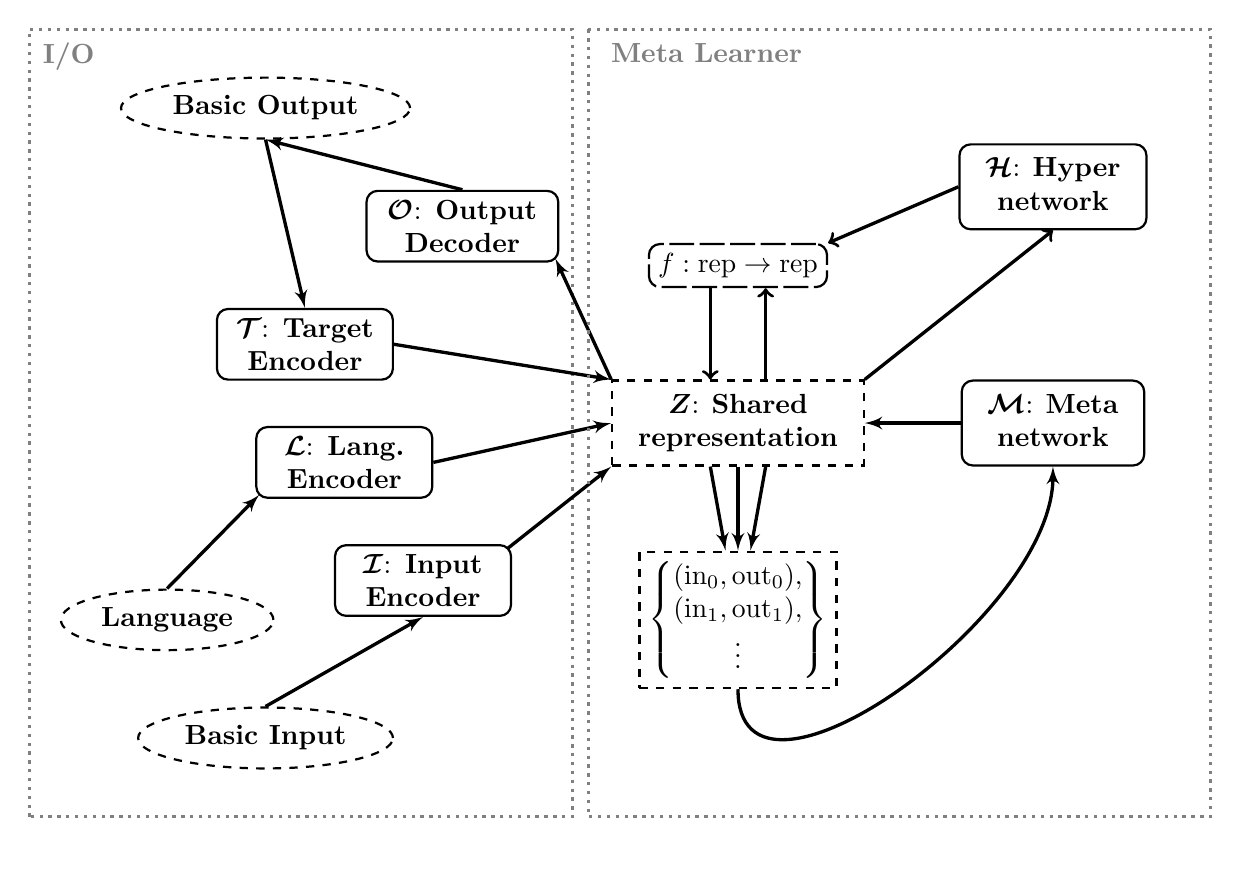
\begin{tikzpicture}[auto]

\node [dashblock] at (0, 0) (rep) {\begin{tabular}{c}$\bm{Z}$: \textbf{Shared} \\ \textbf{representation}\end{tabular}};

% inputs, outputs

\draw [boundingbox] (-9, -5) rectangle (-2.1, 5);
\node [text=gray] at (-8.5, 4.65) {\textbf{I/O}};

\node [conc] at (-6, -4) (perc) {\textbf{Basic Input}};
\node [conc] at (-7.25, -2.5) (lang) {\textbf{Language}};
\node [conc] at (-6, 4) (act) {\textbf{Basic Output}};
\node [block, text width=2cm] at (-4, -2) (IE) {$\bm{\mathcal{I}}$: \textbf{Input Encoder}};
\node [block, text width=2cm] at (-5, -0.5) (LE) {$\bm{\mathcal{L}}$: \textbf{Lang. Encoder}};
\node [block, text width=2.2cm] at (-3.5, 2.5) (OD) {$\bm{\mathcal{O}}$: \textbf{Output Decoder}};
\node [block, text width=2cm] at (-5.5, 1) (TE) {$\bm{\mathcal{T}}$: \textbf{Target Encoder}};
\path [line] (perc.north) to (IE.south);
\path [line] (lang.north) to ([xshift=0.05cm, yshift=0.05cm]LE.south west);
\path [line] ([xshift=-0.05cm, yshift=-0.05cm]IE.north east) to (rep.south west);
\path [line] (LE.east) to (rep.west);
\path [line] (rep.north west) to ([xshift=-0.05cm, yshift=0.05cm]OD.south east);
\path [line] (OD.north) to (act.south);
\path [line] (act.south) to (TE.north);
\path [line] (TE.east) to (rep.north west);

% meta
\draw [boundingbox] (-1.9, 5) rectangle (6, -5);
\node [text=gray] at (-0.4, 4.7) {\textbf{Meta Learner}};

\node [dashblock] at (0, -2.5) (collection) {
\(\left\{
\begin{matrix}
(\text{in}_0, \text{out}_0),\\
(\text{in}_1, \text{out}_1),\\
$\vdots$
\end{matrix}\right\}\)};
\path [line] (rep.south) to (collection);
\path [line] ([xshift=-1em]rep.south) to (collection);
\path [line] ([xshift=1em]rep.south) to (collection);

\node [block] at (4, 0) (meta) {\begin{tabular}{c}$\bm{\mathcal{M}}$: \textbf{Meta} \\ \textbf{network}\end{tabular}};
\path [line] (collection.south) to [out=-90, in=-90] (meta.south);
\path [line] (meta.west) to (rep.east);

% hyper

\node [block] at (4, 3) (hyper) {\begin{tabular}{c}$\bm{\mathcal{H}}$: \textbf{Hyper} \\ \textbf{network}\end{tabular}};
\node [block, dash pattern=on 9pt off 2pt] at (0, 2) (transform) {\(f: \text{rep} \rightarrow \text{rep}\)};

\path [draw, ->, very thick] (rep.north east) to (hyper.south);
\path [draw, ->, very thick] (hyper.west) to (transform.north east);
\path [draw, ->, very thick] ([xshift=-1em]transform.south) to ([xshift=-1em]rep.north);
\path [draw, ->, very thick] ([xshift=1em]rep.north) to ([xshift=1em]transform.south);

\end{tikzpicture}
\caption{Schematic of our general architecure. Blocks with solid edges denote deep networks with learnable parameters, dashed edges represent inputs, outputs, embeddings, etc., and $f$ is a deep network with parameters specified by $\mathcal{H}$.} \label{architecture_fig}
\end{figure}
More formally, we take a \textbf{functional} perspective on learning. A datum can be represented by a constant function which outputs it. (For example, each point in the latent space of an autoencoder can be thought of this way.) This allows us to interpret model inputs or outputs as functions. \par
We can then interpret most machine learning tasks as a mapping of functions to functions. These functions could represent data\footnote{Where ``data'' is a quite flexible term. The approach is relatively agnostic to whether the learning is supervised or reinforcement learning, whether inputs are images or natural language, etc.}, or they could be functions that operate on functions themselves. Under this perspective, learning tasks and learning to flexibly map between tasks, or learning to map from language to tasks, are all the same type of problem. \par
Specifically, we embed inputs, targets, and mappings into a shared representational space $Z$. Inputs are embedded by a deep network $\mathcal{I}: \text{input} \rightarrow Z$. Outputs are decoded from the representational space by a deep network $\mathcal{O}: Z \rightarrow \text{output}$. Targets are encoded by a deep network $\mathcal{T}: \text{targets} \rightarrow Z$. (Targets do not necessarily need to be output-like, e.g. in our RL tasks, we use (action, outcome) tuples as ``targets.'') \par
Given this, the task of mapping inputs to outputs can be framed as trying to find a transformation of the representational space that takes the (embedded) inputs from the training set to the (embedded) targets. These transformations are performed by a system with the following components:
\begin{itemize}
\item $\mathcal{M}: \{(Z, Z), ...\} \rightarrow Z $ -- the meta network, which takes a set of (input embedding, target embedding) pairs and produces a function embedding.
\item $\mathcal{H}: Z \rightarrow \text{parameters}$ -- the hyper network, which takes a function embedding and produces a set of parameters.
\item $f: Z \rightarrow Z$ -- the transformation, implemented by a deep network with parameters specified by $\mathcal{H}$.
\end{itemize}
See Fig. \ref{architecture_fig} for a schematic of the architecture. \par
\textbf{Operation:} A basic forward pass through the system might look as follows.
\begin{enumerate}
\item A training dataset of (input, target) pairs is embedded by $\mathcal{I}$ and $\mathcal{T}$ to produce a set of paired embeddings. Another set of (possibly unlabeled) inputs is provided and embedded.
\item The meta network $\mathcal{M}$ maps the set of embedded (input, target) pairs to a function embedding.
\item The hyper network $\mathcal{H}$ maps the function embedding to parameters for $f$, which is used to transform the second set of inputs to a set of output embeddings.
\item The output embeddings are decoded by $\mathcal{O}$ to produce a set of outputs.
\end{enumerate}
To write this explicitly, suppose we have some dataset of input, target pairs ($D_1 = \{(x_0, y_0), ...\}$), and some input $x$ for which we wish to generate a predicted output $\hat{y}$. This output would be generated as follows:
$$\hat{y} = \mathcal{O}\left(f_{D_1}\left(\mathcal{I} \left(x\right)\right) \right)$$
where $f_{D_1}$ is the transformation the meta-learner guesses for the training dataset $D_1$:
$$f_{D_1} \text{ is parameterized by } \mathcal{H}\left(\mathcal{M}\left( \left\{\left(\mathcal{I}\left(x_0\right), \mathcal{T}\left(y_0\right) \right), \left(\mathcal{I}\left(x_1\right), \mathcal{T}\left(y_1\right) \right), ... \right\}\right)\right)$$
This system can be trained end-to-end if labels are provided for a second set of inputs. In particular, suppose we have some loss function $\mathcal{L}(y, \hat{y})$ defined on a single target output $y$ and actual model output $\hat{y}$, for some input $x$. We define our total loss computed on some dataset $D_2$ as:
$$\mathbb{E}_{(x, y)\in {D}_2} \left[ \mathcal{L}\left(y, \mathcal{O}\left(f_{D_1}\left(\mathcal{I} \left(x\right)\right) \right)\right)\right]$$
More generally, suppose we have some input which is already embedded in the representation space $z_{in} \in Z$, and an embedded dataset $D_Z$ of (embedding, target embedding) pairs $\{(z_{in,0}, z_{out,0})\}$. Then we can generate an output $\hat{z}_{out} \in Z$ as:
$$\hat{z}_{out} = f_{D_Z}(z_{in}) \qquad \text{where } f_{D_Z} \text{ is parameterized by } \mathcal{H}\left(\mathcal{M}\left(D_Z\right)\right)$$
This output can then be appropriately dispatched depending on the task at hand. For example, if the $z_{in,i}$ are the system's embeddings for trying to win various games, and the $z_{out,i}$ are the corresponding embeddings for trying to lose those games, then $z_{out}$ could be interpreted as the system's guess at a losing strategy for the game embedded as $z_{in}$, and then could be used to play that game. We could then evaluate performance by how well the system actually performs at losing with the $z_{out}$ strategy. \par
Similarly, we could map from language to a task embedding, and then ask how well the system performs at the task specified by language. The key feature of our architecture -- the fact that tasks, data, and language are all embedded in a shared space -- allows substantial flexibility within a unified system.



\subsubsection{Results \& future directions}

\textbf{Results:} Briefly, the system is able to do meta-learning in a toy card-game domain I've constructed, that is, it's able to learn a held-out game from seeing a single batch of examples. It's also able to do mapping of tasks, such as trying to lose (based on task-mapping examples), even on held-out games. It can also achieve some success at these behaviors based on natural language input, although it generalizes less well from that than from examples. This is not too surprising, as the structure of a task is more directly captured by examples than by a symbolic encoding. \par 
\textbf{Future directions:}
There are a number of future directions I would like to explore:
\begin{itemize}
\item Can we find a task that demonstrates the ability of this architecture to perform comparably to humans, like OmniGlot \citep{Lake2015} but for more general flexibility?
\item Is there a way we can do unsupervised learning in the latent representation space that would approximate something like rerepresentation \citep{Karmiloff-Smith1986}? Could we do something to generate hypotheses or interesting experiments for active learning \citep{Markant2014a}? 
\item We've assumed knowledge of which experiences come from which tasks. However, this is an important learning problem in its own right, and it would be nice to try to solve it as well, perhaps with an approach similar to \citep{Achille2018}. 
\end{itemize}


\subsection{Towards a better understanding of human transfer and flexibility}
\begin{figure}
\centering
\begin{subfigure}[t]{0.5\textwidth}
\includegraphics[width=\textwidth]{figures/graph_transfer/three_rooms.png}
\captionsetup{width=.9\linewidth}
\caption{Modular structure: this structure contains three distinct clusters with much stronger connectivity within each cluster than between.}
\end{subfigure}%
\begin{subfigure}[t]{0.5\textwidth}
\includegraphics[width=\textwidth]{figures/graph_transfer/fixed_random.png}
\captionsetup{width=.9\linewidth}
\caption{Randomly generated structure: This structure is randomly generated subject to the constraints that it have the same number of nodes and edges as the modular structure, and that each node have degree at least 2.}
\end{subfigure}%
\caption{The graph structures we intend to use in our transfer experiment.}
\label{graph_struct_fig}
\end{figure}
In this section I propose a set of behavioral experiments that will help us to probe the extent of human ability to transfer knowledge within an experimental session. This work builds off of work showing that humans can learn artificial grammars \citet{Cleeremans1991}, and can transfer this knowledge to isomorphic grammars with novel symbols \citep{Tunney2001}. It also builds off work on more complex graph-structure learning, starting with work by Anna Schapiro and colleagues \citep{Schapiro2013}, and continuing to more recent work showing that some graph structures are more learnable than others \citep{Kahn2018}. \par
The proposed experiment is as follows. We will have subjects perform two different tasks. The first will be analogous to the initial learning stage in \citet{Kahn2018}, and will consist of subjects trying to press key combinations in response to lit patterns of squares. Unbeknownst to them, these stimuli will come from a random walk on a structured graph. \citet{Kahn2018} showed that participants implicitly learned about the structure of this graph. After the first part of the experiment, participants will advance to a second part. This will be essentially analogous to the first, except that the cover task will be hitting single letters displayed on the screen, as in \citep{Cleeremans1991}. \par
We will experimentally manipulate the underlying graph structure which generates subjects stimuli in each stage of the experiment. In the first stage, subjects may either experience the modular structure of \citep{Schapiro2013} or a random graph which has the same number of nodes and edges (this will be randomly generated but fixed across subjects). See Fig. \ref{graph_struct_fig} for diagrams of the two structures. The structure in the second task will be crossed with this in a 2 x 2 design. We can thus examine whether there is a benefit to learning the second struture (i.e. more rapid learning and/or fewer mistakes) after an isomorphic graph as opposed to a non-isomorphic one.  \par
Finally, because I am interested in flexibility, we will also assess subjects' ability to explicitly reason about the structures they encountered. Specifically, we will reveal that the stimuli were generated from a structure, and give a subjects a two-alternative forced choice between the two structures, and ask them to pick which one they experienced in the second part of the experiment. We will also ask them to place the stimuli they encountered on this graph, and then evaluate how well they were able to explicitly reconstruct the true structure. \par

\subsubsection{Results and implications}
I believe this is an interesting study for a number of reasons. First, if we see transfer at the level of procedural performance, it will allow us to increase the upper bound on the complexity of structures which can be transferred over a short time scale. Prior work has shown that structures of this complexity can be learned, and that simpler structures can be transferred, but we are not aware of any work showing transfer effects with structures of this complexity. Second, the question of how we can reuse implicitly learned knowledge explicitly is underexplored. If subjects are not at chance on our explicit reasoning outcome measures, it will be interesting to investigate what predicts their performance on these questions. Both of these outcomes will help us to elucidate what sort of flexibility humans have when learning complex structures over short time scales. \par 
Furthermore, this work may have other implications for the literature. For example, \citet{Kahn2018} interpreted their results as showing that some structures are inherently more learnable than others. However, if we observe transfer benefits, an alternative interpretation would be that those results are due to the presence of structures more like this (hierarchical, clustery) in the world rather than any inherent learnability advantages. \par


\section{Reading notes/literature to incorporate(?)}
%%\subsection{Machine learning}
\begin{itemize}
%% Adversarial
\item Adversarial reprogramming of neural networks -- A cool twist on adversarial examples: the authors were able to "hijack" a variety of networks to perform tasks which were somewhat different from the ones they were trained for by creating an input that consisted of a "program-specifying" perturbation and the data for the new task, and then learning a mapping from the hijacked network's outputs to the new outputs. This is a much stronger (and weirder) kind of transfer than many others, suggesting that the networks are performing deeply non-linear computations and that changes in the inputs can richly explore the space of functions that the networks can compute (i.e. suggesting that the networks are quite chaotic systems). The particular examples they chose share a few more features than I would like (i.e. they are all visual tasks), but nevertheless the results are pretty cool. \citep{Elsayed2018}
\item Adversarial examples that fool both computer vision and time-limited humans -- Shows large-perturbation adversarial examples to humans, and under time-pressure they are more likely to make the same mistakes as the networks. More precisely, the adversarial perturbations systematically reduce performance, whereas a simple change of the adversarial permutation (flipping it vertically) leaves performance mostly unaltered. Furthermore, if they are given a 2AFC where the true class is \textbf{not present} they are systematically biased toward the adversarially targeted class. Under no time pressure, humans accurately classify the images.
%% Transfer & non-RL meta-learning 
\item Label efficient learning of transferable representations across domains and tasks -- Throws together a bunch of tricks for the goal of doing transfer learning with a small amount of data, but the key one is using an adversarial discriminator across the hidden layers of the networks performing the different tasks. Aligning the representations in this way appears to substantially improve transfer. (It's probably crucial here that the transfer network is initialized with the parameters of the source network.) \citep{Luo2017} 
\item An overview of multi-task learning in deep neural networks -- 2017 review of the multi-task learning literature in both simpler machine learning models like SVMs and in deep nets, arguing that soft parameter sharing methods of various kinds are underused compared to ``hard'' parameter sharing as with multi-head outputs, e.g.\citep{Ruder2017} 
\item Identifying beneficial task relations for multi-task learning in deep neural networks -- For 10 NLP tasks, this paper trains both single task models and all task pairings, and then exams the extent of transfer for them, and its predictability. They make the claim that ``multi-task gains are more likely for target tasks that quickly plateua with non-plateauing auxiliary tasks,'' with the suggestion that this helps them keep from getting stuck in local minima (saddle-points?). Obviously the complexity of the target task (here number of labels) is also relevant, but also the entropy of the labels in the auxiliary task is positively associated with transfer, i.e. more uniform auxiliary tasks are more likely to yield transfer (less biasing? just more information?). They say something suggestive about being surprised thatt Jensen-Shannon divergences were not particularly predictive features, but they computed them not between tasks as I would have expected but within-task between word train and val frequency distributions.  \citep{Bingel2017}
\item When is multitask learning effective? Semantic sequence prediction under varying data conditions -- Tries frequency and morpho-syntactic auxiliary tasks for semantic NLP tasks, finds that benefits come mostly from auxiliary tasks with \emph{high entropy} and \emph{low skewness}, and that most main tasks don't benefit much (because semantics and syntax are sufficiently separable?). Note that the tasks that do benefit are often the most complex ones and/or ones like question answering where syntax could be highly relevant. \citep{Alonso2017} 
\item Few-shot autoregressive density estimation -- Uses an autoregressive (PixelCNN) approach with attention over source images to meta-learn generalization on Omniglot like tasks (i.e. see a few samples from a distribution, try to generate more from it). This is like GANs, but with an overarching prior distribution that is slowly learned, while you are rapidly generalizing over conditional sub-distributions. Nice work, but more or less the usual meta-learning trick applied to some different visual architectures. \citep{Reed2018}
\item Meta learner with linear nulling -- An approach to meta-learning (demonstrated on few-shot visual recognition) that intuitively involves doing a on-the-fly computed projection of the embedding vectors for each task. More specifically, the embedding is computed such that every example's embedding is closer (cosine similarity) to the weights in its category than to the weights that decode other exemplars, via a null-space projection on an operator defined by the differences between these. Essentially, this is trying to separate the examples along dimensions where the weights are \emph{null to within category variations}. It's a neat little trick, and seems to improve performance on complex tasks. It seems like there might be simpler ones that would work too, I wonder if they have been tried. \citep{Yoon2018}
\item Neural task programming: learning to generalize across hierarchical tasks -- A neural programmer-interpreter derivative that does learning of hierarchical task structure from demonstrations, using a few clever extensions including learned demonstration subsequence selection for sub-tasks, and getting rid of LSTMs in the controller to avoid getting ``stuck'' in incorrect action trajectories if the environment doesn't respond exactly as expected.
\item Probabilistic model-agnostic meta-learning -- An extension of MAML that involves 1) adding noise to the fast-adaption gradients and 2) doing variational inference in order to make this sample from a posterior over possible models. They show that this gives kinda reasonable samples from posteriors over models of some toy (and one non-toy) datasets.  
\item Meta Networks -- Fairly vanilla meta learning but with both fast (i.e. hyper-network-specified) and slow (trained by gradient descent) weights in both the meta learner and task learner, and with the meta learner seeing gradient info from the task learner. Equals human performance on omniglot.
\item Meta-learning for semi-supervised one-shot classification -- Does this obvious thing(s) for integrating unlabeled examples into few-shot classification learning: try to estimate based on the labeled examples what each classes distribution is, and then softly include the unlabeled examples according to their likelihood under those distributions. More generally, have a neural net learn how to figure out whether to include examples based on various statistics about the distributions.
\item Zero-data learning of new tasks -- Learning tasks from purely linguistic (or other symbolic) descriptions. They consider both just giving a task description as input like any other and conditioning the model on it directly (in the standard sort of meta-learning way, with a Bayesian discriminator), in their most interesting model by taking a learned feature-processor and conditioning the output weights on the description. It works decently, as one would expect, on the few relatively-simple tasks they tried. 
\item Image to image translation for domain adaption -- Uses consistency along a bunch of different paths (cycles and beyond, so related to consistency things I've thought about) to do domain adaptation of images for training, e.g. from video game driving scenes to real street scenes. Really just applies a bunch of different things that had been done previously with tuned weights, but gets pretty good results.
\item PathNet: Evolution Channels Gradient Descent in Super Neural Networks -- Uses network of modules (smaller nets) to learn task, evolves which modules to uses then fixes the most useful ones. By reinitializing other modules, and learning from this starting point, they are able to achieve transfer benefits on a variety of tasks. \citep{Fernando2017}
\item Learning to Make Analogies by Contrasting Abstract Relational Structure -- Does a simple Raven's Progressive Matrices analog where a network sees a ``source'' sequence that obeys some relationship, and then sees a ``target'' sequence, and has to figure out what the last element of the target sequence should be from a set of candidates. They show that if the false candidates contrast different possible relationships (as opposed to randomly sampled), the network seems to learn abstract features and generalize better. Obviously relates to curriculum and active sampling issues. \citep{Hill2019}
%% RL
\item A deep hierarchical approach to lifelong learning in minecraft -- Does mostly obvious tricks to incorporate options (in the RL sense) into DQN-style learning -- learns options as (possibly distilled) indepndent subnetworks, learns a policy for choosing whether to use a primitive action or an option, and then follows options until a (learned) termination criterion. For all that fancy architecture, it still doesn't have either the flexibility to compose skills or learn more than a fixed number of skills, and the results are far from astonishing. \citep{Tessler2016}.
\item RL$^2$: Fast reinforcement learning via slow reinforcement learning -- The standard deep-learning meta-learning tricks applied to RL. Instead of running an RL algorithm on a single task, train an RL algorithm such that it does well at choosing the next action on *any* given MDP from the sequence of previous states it has seen in that MDP, much as a human might learn to perform quite well on a videogame based on their previous experiences in it. The network does this in the most obvious way: just slap some recurrence in your policy network which maps from (S, A, R, S) tuples to actions and let gradient descent sort the rest out. Works pretty well on some toy non-toy tasks (relatively simple tasks dressed up with high-dimensional input and action spaces).
\item Learning to reinforcement learn -- Much like the RL$^2$ paper above, slaps some recurrence in a network which maps from (S, A, R) tuples to policy and value estimates, and then trains it to do well across episodes drawn from a distribution of tasks, then shows that it generalizes and can even show ``model-like'' behavior, in the sense that it will one-shot learn to take actions which lead to more rewarding states, that is, it seems to have learned to integrate observed transitions and rewards into its decisions on the fly. 
\item Guided cost learning: deep inverse optimal control via policy optimization -- One type of efficient learning that humans can do is learning from demonstrations. The problem of inferring an objective function from a demonstration is know as the inverse RL problem in the RL literature. This paper presents an algorithm for this based on inferring the objective and policy at the same time (instantiating at least the objective as a deep net) and demonstrates the success of the algorithm in robotics. \citep{Finn2016}
\item Meta learning shared hierarchies -- A kinda hacky (but intuitively reasonable) approach to shared-option meta-learning where \(k\) different option policies are learned, and then on each task a (task-specific) master policy is learned which just chooses between them. On a new task, they burn-in updates of the master policy to get semi-reasonable performance, and then do alternate updating of the option policies and the master policy. It does pretty reasonably well when you can assume that all your options should be shareable between tasks, but it's not clear how applicable it would be to domains where this is not true. It also doesn't pass any gradients between the master and option policies which (as they themselves admit) probably makes learning complex things more difficult. Also only one level of hierarchy, as usual. \citep{Frans2018} 
\item Some considerations on learning to explore via meta-reinforcement learning -- Proposes to make meta-RL systems do better at exploring by explicitly accounting for it in the loss. Gives modifications of MAML and $RL^2$. For MAML they add an additional loss term which rewards actions in an initial (hard-coded) exploratory phase which increase the rewards later (they don't see much improvement from this, and my guess is that it's because it's really hard to estimate this loss term). For $RL^2$ they just zero out the loss from the initial exploratory period, which seems to work pretty well. Both methods do better than (either) baseline in general. Interestingly their modification of $RL^2$ is generally the best asymptotically (in meta training) even though the $RL^2$ baseline is much worse than either MAML or their modification of it.
\item Life-Long Disentangled Representation Learning with Cross-Domain Latent Homologies -- Essentially an extension of a VAE that classifies inputs as coming from different environments and tries to learn (partially overlapping) latent dimensions which explain those data, doing some masking of dimensions that seem irrelevant for the present example so they don't get biased, and using replay (hallucination based on old parameters rather than actually keeping memories) to prevent catastrophic interference. \citep{Achille2018}
\item Neural Episodic Control -- Nonparametric DQN, essentially. Instead of computing Q-values parametrically from state representation, stores memories of previous state representations and Q-values, and then uses those to produce similarity-weighted Q-value estimates for new states. This learns fatster (and often does better) than parametric models. \citep{Pritzel2017}
%% NLP or "symbolic" architectures
\item Relational inductive biases, deep learning, and graph networks -- Argues that we should build networks that have graph-structured inductive biases about the world, given that the world has relational structure and (insert Gentner here) says it's super important for our reasoning. They propose a general type of networks like this which update as follows: each edge is updated depending on its state, its endpoints states, and the graph state;, each vertex is updated depending on its state, its edges' states, and the graph state; and finally the graph state is updated depending on its state and all its vertices' states. Relates this to an number of other graph/set networks that have been proposed recently. They suggest composing these graph-network blocks much like one would compose layers in a standard neural net, including the possibility of things like recurrence. (However, the constraint of ``things must be the same size'' to be combined in a standard net scales to the much more limiting constraint of ``things must be the same graph'' in this architecture -- this may not be devastating, but isn't there a better way?) They argue that networks built on these principles, because they reuse computations in a way that respects graph structures, will generalize more robustly to new situations. They cite a number of papers that prove this in the case of generalizing to e.g. larger graphs (``combinatorial generalization''). However, they point out that their invariance to node permutations makes certain kind of graph computations difficult, and furthermore that graphs do not make ideas like recursion easy to represent. Furthermore, the type of combinatorial generalization they show is still far from the flexibility of human intelligence.\citep{Battaglia2018} 
\item DARTS: Differentiable Architecture Search -- It's not actually full architecture search that is differentiable, but more searching for blocks (like Inception blocks). The basic idea is very simple: just use a softmax over all possible operations (e.g. conv, pooling, etc.). This is then differentiable, but they are being tricky and optimizing the architecture with respect to the validation loss after a single step of gradient descent on the weights using the train data. Because of this, they find that first order optimization of the architecture alone is insuffficient, so they approximate the second derivative with a finite difference weighted by a tunable parameter, and it works well enough for their purposes. An interesting step towards differentiable architecture search, and they show it speeds up learning certain kinds of cells quite a bit, but the title oversells it a bit I think.  
\item Tensor Product Generation Networks for Deep NLP Modelling -- Implements a NLP architecture that allows for (but does not necessitate) tensor-product-representation-like ``unbinding'' of fillers from roles, achieves state of the art on MSCOCO captioning with it, and then shows that the unbinding vectors are actually fulfilling at least some grammatical functions (although there is probably more mixed in there, and they certainly don't show that they're handling all the grammatical functions, just that they mostly cluster nicely by certain grammatical features).
\item Symbolic functions from neural computation -- Starts from the basic ideas of tensor product representations and symbols as encoded as patterns of activation in an (infinite-dimensional) vector space, and shows some surprisingly complex computations, such as recursive access to node information or children in binary trees, or various grammatical rules, can be reduced to \emph{linear} transformations within these vector spaces.  
\item Optimization and quantization in gradient symbol systems: a framework for integrating the continuous and discrete in cognition -- Essentially a more readable follow-up to \citep{Smolensky2006} above, which goes on to argue that the way to have discrete output attractors from a continuous system is to have essentially seperate \emph{optimization} (continuous, via SGD) and \emph{quantization} (soft discretization), and linearly interpolate from the former to the latter over processing time. Argues that this makes good quantitative predictions about speed accuracy tradeoffs, e.g. \citep{Smolensky2014}
\item Learning and analyzing vector encoding of symbolic representations -- A short paper reviewing some methods of symbol binding in neural nets and proposing to just throw LSTMs at the problem instead, and then showing a very weak demonstration that it works (the embedding vectors kinda obey the basic superposition rule you would want them to). \citep{Fernandez2018} 
\item Improved semantic representations from tree-structured long short-term memory networks -- Points out that there's no reason for the simple chain-style graphs of typical recurrent networks, any DAG will do. In particular, they build tree-structured networks on the fly from various parse trees (constituency and dependency) of sentences, and show that processing the inputs through these networks yields better performance than basic LSTMs on a sentiment and semantic tasks. \citep{Tai2015} 
\item Ask me anything: dynamic memory networks for natural language processing -- Proposes a fairly complicated memory based architecture for NLP tasks like bAbI. Basically, the model consists of a probe encoder, the probe embedding is then used as attention over the input to generate ``episodic'' encodings of each input chunk (sentence or word depending on the task) of the input. Then the memory network does a fixed number of passes of episodic ``recall'' conditioned on 1) the question, and 2) the previously recalled memory, via a GRU with (atypical) attention based on the episode, the previous memory, and the question. The final memory produced is passed as input to the answer module, along with the question. This architecture slightly outperforms simpler architectures at most tasks (including the paper above at sentiment analysis). \citep{Kumar2015}
\item Learning with Latent Language -- Pre-learns what is essentially a simple domain-dependent image-captioning model, and then shows that inferring a latent language description that optimally performs on the task (or better yet, sampling many and taking an average) works better than other meta-learning strategies, even multi-task ones that have language learning during pre-training. But is it because of their uniquely symbol-structured tasks? The RL task doesn't use pixels as input, and they provide direct policy supervision during the pre-training part. \par 
%% Other
\item Insights on representational similarity in neural networks with canonical correlation -- Proposes a simple generalization of CCA based on accounting for the variance explained by each component as well as the correlation. Shows that this captures some interesting features of relationships between neural networks. First, networks that are ``memorizing'' are less similar under this metric than networks that generalize better. Furthermore, even for networks that generalize well, more similar hyperparameters result in more similar representations at end of training, i.e. there is a ``signature'' of the hyperparameter choices made left behind in the representations. They also observe ``bottom-up'' convergence, where the lower layers of networks (including RNNs) get more similar before the later layers do.  
\item On the importance of single directions for generalization -- Ablation/noise robustness of neural networks is related to generalization, networks that memorize more use more ``single directions'' of representation space to encode dimensions. They find that dropout only increases ablation robustness up to the dropout threshold, whereas batch norm substantially increases it. They also find, interestingly, that batch norm substantially decreases class selectivity of any given filter in a CNN, which they suggest explains the previous result. The overall single directions result seems easily explained from Surya's and my generalization theory paper. \citep{Morcos2018}
\item Outrageously large neural networks: the sparsely gated mixture-of-experts layer -- proposes a neural net ``layer'' that consists of many smaller ``expert'' networks (single hidden layer in their examples) that are sparsely selected via importance weights from a top-$k$ selection over a (noisy) softmax based on a learnable linear transform of the input. The model loss includes a term for the coefficient of variation of the importance weights, encouraging many experts to be used (otherwise there is a rich-get-richer problem where the most selected experts become selected even more). Stacking this layer in between LSTMs improves performance on language modeling and translation tasks. \citep{Shazeer2017} 
\item Deep visual-semantic alignments for generating image descriptions -- A paper on image captioning that was one of the first to propose the idea of conditioning RNNs on CNN reps to caption images, and also contains some interesting hints of consistency-based auxiliary tasks based on aligning saliency selected sub-regions of an image (selected for containing objects) with subsets of the caption. \citep{Karpathy2017} 
\item Unsupervised Feature Learning via Non-Parametric Instance Discrimination -- Learns surprisingly good visual features in an unsupervised way by trying to do classification of each instance as separate from others. These features generalize well to classification (in a non-parametric way), but also do better than supervision-generated features at transfer to unseen datasets. \citep{Wu2018}

\end{itemize}

%%\subsection{Cognitive Science}
\begin{itemize}
\item Analogy and abstraction -- A review of analogical reasoning in learning, with a slightly devo focus, exploring phenomena such as superficial similarity driving alignment of domains, how this impacts transfer and when people are able to make more abstract alignments. My (heavily biased) spin on their conclusions is that there is a progression from relations per se to relations-as-objects (cf. Annette Karmilov-Smith) and the claim is that then more abstract relations-among-relations are really just relations among objects which are results of the previous process. \citep{Gentner2017}
\item Similarity and the development of rules -- A review of some of the analogical reasoning literature arguing that similarity (even superficial similarity) is important in abstract reasoning, for example children can learn an abstract relationship more easily if they see superficially similar examples of it first to scaffold it, and the patterns of interference in analogicial reasoning are strongly suggestive of similarity at various levels of abstraction playing a role in reasoning, for both adults and children.
\item A model of learning by incremental analogical reasoning and debugging -- Argues for a process of as-needed structure mapping by directly choosing known structures and doing a top-down matching process that is sensitive to the structural links. It then locally debugs to ``fix'' over-interpretation of the analogy. \citep{Burnstein1983}
\item Learning overhypotheses with hierarchical Bayesian models -- Makes the point that hierarchical Bayesian models can capture learning at different levels of abstraction, acknowledges that the highest level prior must still be built in, but makes the tendentious claim that it can be made simple enough to either be obvious or innate. \citep{Kemp2007}
\item A taxonomy for far transfer -- A review that breaks down transfer studies along axes of content and context (with sub-axes for each) and argues that the disagreement in the literature over whether and to what extent transfer occurs is due to the conflation of these many different types of transfer. Their take, while critical, is generally positive on the existence of far transfer. \citep{Barnett2002}
\item All other things being equal: acquisition and transfer of the control of variables strategy -- Explores teaching the control of variables strategy (i.e. holding everything else constant when testing the effect of one variable) to elementary school children, and seeing how well they're able to apply it and transfer it to new problems (the problems were learning about springs, ramps, and sinking in water). In general, older students did better at both applying and transferring, and students who received explicit instruction as well as probe questions (which made them think about the revelant ideas) did better than students who received only probe questions or nothing. The strategy was transferable to problems that were in some ways superficially different (experimenting on different objects), but where the overall context was similar. Many students in all conditions used (and often mentioned) the strategy at least once. However, relatively few students in any condition were able to explicitly identify the strategy when asked about similarities between the problems. \citep{Chen1999}
\item Statistical learning:  from acquiring specific items to forming general rules. -- Short review arguing that rule-like learning in both adults and children is just statistical learning over appropriate features given the input variability. 
\item Generalization, similarity, and Bayesian Inference -- Bayesian models of category formation and generalization can capture aspects of these phenomena that classical models of Shepherd and others cannot; Priors which assume active sampling of positive examples yield effects like narrowing of CIs (cognitively) around observed exemplars as N increases. \citep{Tenenbaum2001}
\item Two modes of transfer in artificial grammar learning -- Different types of transition features seem to be learned by different processes, or at least processes which are dissociable in terms of how noise affects transfer to novel domains. In particular, repetition is a feature that lends itself to creating abstract ``analogy''-like features which can transfer despite noise (where the transition doesn't always occur even if the first item does), but longer distance pairwise dependencies are very sensitive to noise in co-occurence probabilities. \citep{Tunney2001}
\item Getting symbols out of a neural architecture -- Explores the problem of role-filler binding in neural nets, and argues from basic computational principles that vector addition is the right approach (i.e. have a ``role'' vector and a ``filler'' vector and add them), rather than fancier approaches like outer products, because addition has the right compositional structure for human flexibility. \citet{HummelSomeYear}
\item On the proper treatment of connectionism -- BBS article by Smolensky from the early days of connectionism, articulating a position on the relationship between symbolic and sub-symbolic computation and arguing that emergence is an important and useful way of cognitve function even in highly symbolic domains. Takes a somewhat too discrete dual-systems-like view for my taste, but a good source for old quotes about the relationships between symbols and intuitions in cognition and neural networks. \citep{Smolensky1988}
\item The cognizer's innards: a psychological and philosophical perspective on the development of thought -- Argues for Karmiloff-Smith's \emph{representational redescription} (RR) theory; that we successively create more abstract representations by re-representing our prior knowledge. Points out that connectionist networks typically lack the ability to reason flexibly over their own representations, and suggests that overcoming this may require hybrid models, but points out that they will probably need to be more general than the simple one-level hybrid models that include just one mapping from distributed representations to symbols. Some interesting examples of where to look for evidence of redescription in progress. \citep{Clark1993}
\item From meta-processes to conscious access: Evidence from children's metalinguistic and repair data -- A more detailed review of AKS' theory of representational redescription and the evidence for it from patterns of children's linguistic errors and (sometimes unecessary) repairs and a few other nice examples thrown in. In particular, there is a very nice example of children failing to balance an oddly shaped block when asked to do so, but successfully balancing it when asked to build a house, because \emph{their explicit theory is that blocks balance in the middle, but their procedural knowledge is more sophisticated}, but asking them explicitly to do something calls up their conscious knowledge primarily. Also contains the most explicit statement of her ``model'' in any of her work that I've read to date, although still not close to being a quantitative model. \citep{Karmiloff-Smith1986}
\item How the Abstract Becomes Concrete: Irrational Numbers Are Understood Relative to Natural Numbers and Perfect Squares -- Looks at how people understand irrational numbers (actually only square roots), which the authors apparently consider to be a ``highly abstract'' mathematical concept. They find that people do tasks like magnitude estimation with irrationals by relating them to more easily understood numbers. People who have better strategies for this do better. Their only interesting finding to me is a negative: unlike for natural numbers and rationals, better performance on magnitude-type tasks was not related to more conceptual knowledge about irrationals (but number-line estimation was). Useful as it relates to \citep{Wilensky1991}. 
\item Metaphor: Bridging embodiment to abstraction -- Argues that metaphors allow embodied cognition to extend to more abstract concepts. Is this a useful point or a tautology? 
\item Rule abstraction, model-based choice, and cognitive reflection -- Compares subjects use of more low-level and more abstract strategies on two tasks (feature vs. rule-based generalization of categories, model-free vs. model-based RL) and the cognitive reflection task (which requires overriding a superficially obvious response). Positive associations where they would be expected, partially but not completely mediated by cognitive reflection. Some interesting dissociations, e.g. some subjects could give the rule when prompted but didn't perform in accordance with it. Model-based choice appeared to be related to rule-based generalization, but model-free is independent of it (model-based and model-free make predictions about two different test trials in their task). Their measures are correlational; their conclusions are vague. 
\item The role of gesture in communication and thinking -- Gesturing is found broadly, seems to serve important functions for communication, \textbf{and}, she argues, for the speaker's thinking. \citet{Goldin-Meadow1999}
\item Transitions in concept acquisition: using the hand to read the mind -- Gestures-speech mismatch in children problem-solving signaled readiness to learn a new concept that their gestures were hinting at, though they could not yet state it.
\item Organizing conceptual knowledge in humans with a gridlike code -- Trained subjects to locate points within a two-dimensional ``conceptual'' space (bird leg length and bird neck length). They showed subjects morphs of birds at a specific angle in this space and had them do a categorization task on the outcomes. Found that there was a bias towards hexagonal symmetry in their representations, such that the fMRI signal showed a sinuisoidal modulation with a period of 60 degrees. Furthermore, the degree of this bias was correlated with peformance. They suggest that this means that subjects are relying on grid cell codes to represent even this conceptual space. Obvious grounding connections here, but would this result in any effects that are measurable purely behaviorally? Also, why would subjects necessarily have to scale both dimensions with the same unit? The angles of course depend on that... Is it because these are really both spatial dimensions? \citep{Constantinescu2016}\par
\item How, whether, why: Causal judgements as counterfactual contrasts -- Tobi's billiard-ball causality paper. Worth thinking about how intuitively people understand the necessary/sufficient distinction in this context when they struggle with it in others. (Like the Wason selection task social cover story.) \citep{Gerstenberg2015} \par
\item Medial prefrontal cortex predicts internally driven strategy shifts -- Gave people an explicit but somewhat difficult task, where there was a (non-instructed) feature (color) that was actually a deterministic cue to the correct response. Participants who reported having noticed this showed sharp shifts in behavior, but these shifts were \textbf{preceded} by color being decodable from PFC. Interesting w.r.t. the issue of whether and how implicit statistical learning becomes explicit. However, there's a high chance of this time ordering being artifactual with the way they computed when the behavioral shift occurred. Talked to Paul Muhle-Karbe about possibility of running an interrupted behavioral paradigm to try to get a bit more traction. \citep{Schuck2015} \par
\item Learning the structure of event sequences -- Jay \& Axel's paper on implicit learning of grammars \citep{Cleeremans1991}.
\item Network constrainsts on learnability of probabilistic motor sequences -- Paper Danielle Bassett talked about in MBC with how graph structure affects implicit learning a la Schapiro or Cleeremans. \citep{Kahn2018} 

\item Training the approximate number system improves math proficiency -- Causally experiment showing that ANS training with adding and subtracting dot arrays improves scores on symbolic addition and subtraction!! \citep{Park2013}
\item Improving arithmetic performance with number sense training: an investigation of an underlying mechanism -- Digs deeper into the above results, showing that other kinds of targeted training don't help, and doing an \textit{okay} (non-)control  experiment showing that verbal suppression doesn't interfere with the ANS task (but not actually showing that it doesn't interfere with the transfer effect to symbolic). \citep{Park2014}
\end{itemize}

Some assorted William James quotes:
\begin{itemize}
\item ``But what are now the defects of the nervous system in those animals whose consciousness seems most highly developed? Chief among them must be instability. The cerebral hemispheres are the characteristically 'high' nerve-centres, and we saw how indeterminate and unforeseeable their performances were in comparison with those of the basal ganglia and the cord. But this very vagueness constitutes their advantage. They allow their possessor to adapt his conduct to the minutest alterations in the environing circumstances, any one of which may be for him a sign, suggesting distant motives more powerful than any present solicitations of sense. It seems as if certain mechanical conclusions should be drawn from this state of things. An organ swayed by slight impressions is an organ whose natural state is one of unstable equilibrium. We may imagine the various lines of discharge in the cerebrum to be almost on a par in point of permeability - what discharge a given small impression will produce may be called accidental, in the sense in which we say it is a matter of accident whether a rain-drop falling on a mountain ridge descend the eastern or the western slope. It is in this sense that we may call it a matter of accident whether a child be a boy or a girl. The ovum is so unstable a body that certain causes too minute for our apprehension may at a certain moment tip it one way or the other. The natural law of an organ constituted after this [p.140] fashion can be nothing but a law of caprice. I do not see how one could reasonably expect from it any certain pursuance of useful lines of reaction, such as the few and fatally determined performances of the lower centres constitute within their narrow sphere. The dilemma in regard to the nervous system seems, in short, to be of the following kind. We may construct one which will react infallibly and certainly, but it will then be capable of reacting to very few changes in the environment - it will fail to be adapted to all the rest. We may, on the other hand, construct a nervous system potentially adapted to respond to an infinite variety of minute features in the situation; but its fallibility will then be as great as its elaboration. We can never be sure that its equilibrium will be upset in the appropriate direction. In short, a high brain may do many things, and may do each of them at a very slight hint. But its hair-trigger organization makes of it a happy-go-lucky, hit-or-miss affair. It is as likely to do the crazy as the sane thing at any given moment. A low brain does few things, and in doing them perfectly forfeits all other use. The performances of a high brain are like dice thrown forever on a table. Unless they be loaded, what chance is there that the highest number will turn up oftener than the lowest?'' -- The Principles of Psychology, Ch. 5.
\end{itemize}


\bibliographystyle{apalike}
\bibliography{arrr}
\end{document}
